
\serie{Vocabulaire}

\begin{exercice}[Dans la vie courante]
Donne des exemples de la vie courante pour lesquels on utilise :
\begin{enumerate}
 \item Des nombres entiers relatifs ;
 \item Des nombres relatifs non nécessairement entiers.
 \end{enumerate}
\end{exercice}


\begin{exercice}[Interprétation]
Parmi la liste de mots suivants, quels sont ceux qui peuvent « se traduire » à l'aide : 
\begin{enumerate}
 \item D'un nombre relatif positif ?
 \item D'un nombre relatif négatif ?
 \item Du nombre relatif « 0 » ?
 \end{enumerate}
 
Diminuer, croître, soldes, monter, croissance, recul, freiner, augmenter, déclin, progression, ajouter, hausse, maigrir, ôter, dépense, régression, stable, descendre, accélérer, baisse, centupler, fixe, atténuer, constant, restreindre, chute, ascendant, amoindrir, stagnation.
\end{exercice}


\begin{exercice}
Recopie et complète les phrases en utilisant les mots proposés :

\boxed{positif} \quad \boxed{négatif} \quad \boxed{plus} \quad \boxed{relatif} \quad \boxed{relatif}.

\begin{enumerate}
 \item $- 4$ est un nombre \ldots \ldots \ldots \ldots ;
 \item Un nombre \ldots \ldots \ldots \ldots peut s'écrire sans le signe \ldots \ldots \ldots \ldots ;
 \item L' \ldots \ldots \ldots \ldots d'un nombre relatif \ldots \ldots \ldots \ldots est un nombre relatif \ldots \ldots \ldots \ldots ;
 \item $+ 3$ est l' \ldots \ldots \ldots \ldots de $- 3$.
 \end{enumerate}
\end{exercice}


\begin{exercice}[L'opposé de l'opposé]
\begin{enumerate}
 \item Recopie et complète le tableau suivant : \\[0.5em]
 \begin{tabularx}{0.8\linewidth}{|c|X|X|X|X|X|}
  \hline
 Nombre & 5 & & 0 & $- 27$ & \\\hline
 Opposé du nombre & & $- 2$ & & & \\\hline
 Opposé de l'opposé du nombre & & & & & 10 \\\hline
  \end{tabularx} \\[0.5em]
 \item Que peux-tu dire de l'opposé de l'opposé d'un nombre relatif ?
 \end{enumerate}
\end{exercice}


\begin{exercice}[Classement]
Soient les nombres relatifs suivants :
\begin{colitemize}{3}
 \item $- 7,8$ ;
 \item $+ 13$ ;
 \item 0 ;
 \item $- 7,3$ ;
 \item $- 0,07$ ;
 \item $- 0$ ;
 \item $+ 2005$ ;
 \item $- \dfrac{27}{5}$ ;
 \item 0,0001 ;
 \item 18,43 ;
 \item $+ 1979$.
 \end{colitemize}
 
Classe ces nombres relatifs en deux catégories :
\begin{itemize}
 \item Les négatifs ;
 \item Les positifs.
 \end{itemize}
Quel(s) nombre(s) se trouve(nt) dans les deux catégories ?
\end{exercice}


\begin{exercice}[Hauteurs et profondeurs]
Sur ton cahier, reproduis l'axe gradué ci-contre sur lequel 1 cm correspond à 500 m puis place, le plus précisément possible, les hauteurs et profondeurs suivantes :

\begin{minipage}[c]{0.8\linewidth}
\begin{itemize}
 \item \textbf{A} : le Chasseral est un sommet du Jura qui est situé à 1\,607 mètres d'altitude ;
 \item \textbf{B} : le Tibet est le plus haut plateau du monde avec une altitude moyenne de 4\,500 m ;
 \item \textbf{C} : la Mer Morte en Asie a une profondeur de 349 m ;
 \item \textbf{D} : le cachalot peut plonger jusqu'à 700 m pour se nourrir ;
 \item \textbf{E} : la hauteur de la tour Eiffel est 324 m.
 \end{itemize}
 \end{minipage} \hfill%
 \begin{minipage}[c]{0.15\linewidth}
 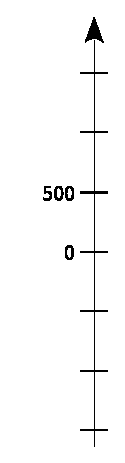
\includegraphics[width=1.2cm]{axe500}
  \end{minipage} \\
\end{exercice}


\begin{exercice}
On considère un immeuble comportant un rez-de-chaussée et cinq étages ainsi qu'un parking en sous-sol avec deux niveaux. 

Dessine le panneau de commandes de l'ascenseur de cet immeuble.
\end{exercice}


%%%%%%%%%%%%%%%%%%%%%%%%%%%%%%%%%%%%%%%%%%%%%%%%%%%%%%%%%%%%%%%%%%
\serie{Repérage sur une droite}

\begin{exercice}[Abscisses]
Pour chaque cas, lis puis écris les abscisses des points $A$, $B$, $C$, $D$ et $E$ :
\begin{enumerate}
  \item \begin{center} 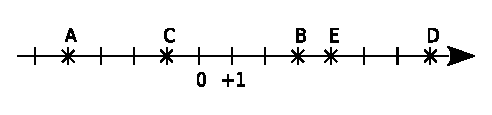
\includegraphics[width=7.4cm]{axeA} \end{center}
  \item \begin{center} 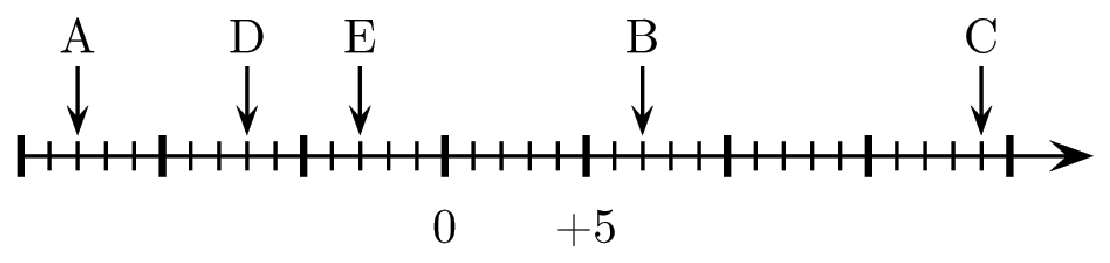
\includegraphics[width=7.4cm]{axeB} \end{center}
  \item \begin{center} 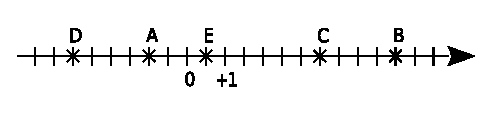
\includegraphics[width=7.4cm]{axeC} \end{center}
  \item \begin{center} 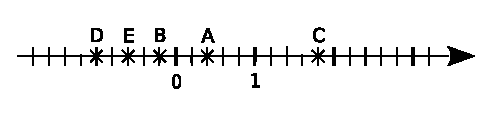
\includegraphics[width=7.4cm]{axeD} \end{center}
  \item \begin{center} 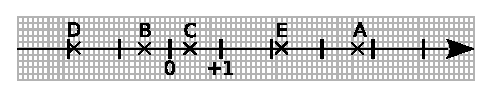
\includegraphics[width=7.4cm]{axeE} \end{center}
 \end{enumerate}
\end{exercice}


\begin{exercice}[Placements de points]
Reproduis les dessins de chaque droite graduée et place les points $A$, $B$, $C$, $D$ et $E$ d'abscisses respectives :

\begin{enumerate}
  \item \begin{center} 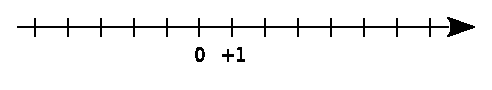
\includegraphics[width=7.4cm]{axeABCDE1} \end{center}
  
 $A(- 1)$ ; $B(+4)$ ; $C(- 3)$ ; $D(+3)$ ; $E(- 5)$. \\[1em]
  \item \begin{center} 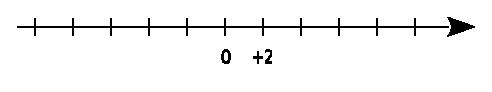
\includegraphics[width=7.4cm]{axeABCDE2} \end{center}
  
 $A(- 2)$ ; $B(+ 4)$ ; $C(- 6)$ ; $D(+ 8)$ ; $E(- 8)$. \\[1em]
  \item \begin{center} 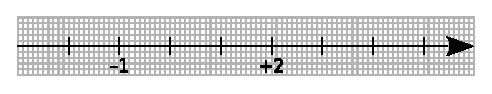
\includegraphics[width=7.4cm]{axeABCDE3} \end{center}
  
 $A(+ 4)$ ; $B(- 0,5)$ ; $C(+ 0,8)$ ; $D(+ 3,4)$ ; $E(- 2,1)$.
 \end{enumerate}
\end{exercice}


\begin{exercice}[Placements de points (bis)]
\begin{enumerate}
 \item Trace une droite graduée en prenant le centimètre comme unité ;
 \item Place sur cette droite les points suivants : 
 
$A(- 5)$ ; $B(+ 3)$ ; $C(+ 2)$ ; $D(- 4)$ ; $E(+ 5)$ ;
 \item Place le milieu $L$ du segment $[AB]$. Lis puis écris l'abscisse du point $L$ ;
 \item Place le point $M$ tel que $C$ soit le milieu du segment $[EM]$. Lis et écris l'abscisse du point $M$.
 \end{enumerate}
\end{exercice}


\begin{exercice}
Trace une droite graduée et choisis une unité convenable pour placer les points suivants :
\begin{colitemize}{4}
 \item $A(52)$ ;
 \item $B(- 36)$ ;
 \item $C(80)$ ;
 \item $D(- 12)$.
 \end{colitemize}
\end{exercice}


\begin{exercice}[Histoires]
\begin{center} 
\includegraphics[width=7.4cm]{axe1000} \end{center}
Reproduis cette droite graduée pour que 5 cm correspondent à 1\,000 ans et place les événements suivants le plus précisément possible :
\begin{itemize}
 \item K : construction de la pyramide de Khéops, vers – 2\,600 ;
 \item J : naissance de Jules César, en – 100 ;
 \item N : début du Nouvel Empire, vers – 1\,550 ;
 \item A : Alexandre le Grand envahit l'Égypte, vers – 350 ;
 \item C : couronnement de Charlemagne, vers l'an 800.
 \end{itemize}
\end{exercice}


\begin{exercice}
Réponds par Vrai ou Faux à chacune des affirmations suivantes et justifie la réponse :
\begin{center} 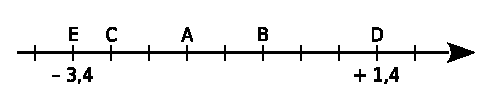
\includegraphics[width=7.4cm]{axeVrai} \end{center}
\begin{enumerate}
 \item Il y a exactement quatre entiers relatifs compris entre les abscisses des points $E$ et $D$ ;
 \item Le point $A$ a pour abscisse $- 1,2$ ;
 \item L'abscisse de $B$ est positive ;
 \item L'abscisse de $C$ est $- 2,8$ ;
 \item L'abscisse du milieu du segment $[AB]$ est un nombre entier relatif positif ;
 \item Exactement deux points ont une abscisse positive.
 \end{enumerate}
\end{exercice}


%%%%%%%%%%%%%%%%%%%%%%%%%%%%%%%%%%%%%%%%%%%%%%%%%%%%%%%%%%%%%%%%%%
\serie{Repérage dans le plan}

\begin{exercice}[Signes des coordonnées]
\begin{minipage}[c]{0.3\linewidth}
Les axes de coordonnées d'un repère partagent le plan en quatre zones, notées $z_1$, $z_2$, $z_3$ et $z_4$.
 \end{minipage} \hfill%
 \begin{minipage}[c]{0.65\linewidth}
 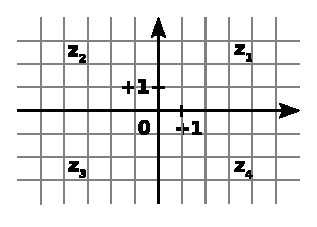
\includegraphics[width=4.6cm]{plan_colore}
  \end{minipage} \\[1em]
Pour chacune des zones, donne le signe de chacune des coordonnées (abscisse et ordonnée) d'un point de cette zone.
\end{exercice}


\begin{exercice}[Lecture de point]
Lis puis écris les coordonnées des points $A$, $B$, $C$, $D$, $E$, $F$, $G$ et $H$ ci-dessous :
\begin{center} 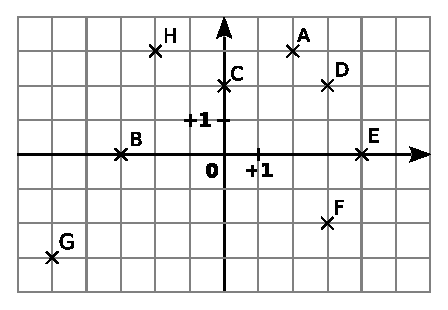
\includegraphics[width=6.7cm]{plan_blanc} \end{center}
\end{exercice}


\begin{exercice}
Lis puis écris les coordonnées des points $A$ à $K$ ci-dessous :
\begin{center} 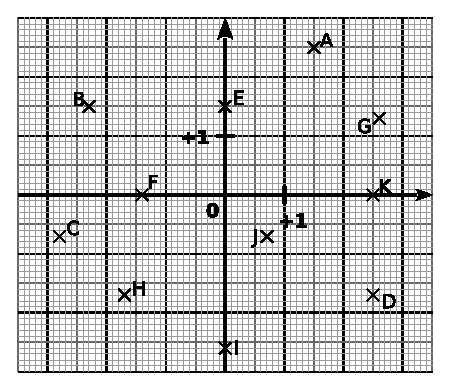
\includegraphics[width=6.7cm]{plan_noir} \end{center}
\end{exercice}


\begin{exercice}
Trace un repère d'unité 1 cm pour chaque axe puis place les 9 points suivants :
\begin{colitemize}{3}
 \item $P(+ 2 ; + 5)$ ;
 \item $R(+ 2 ; - 6)$ ;
 \item $S(- 7 ; + 4)$ ;
 \item $T(- 5 ; - 2)$ ;
 \item $U(0 ; - 4)$ ;
 \item $V(+ 6 ; 0)$ ;
 \item $W(- 3 ; - 5)$ ;
 \item $X(+ 2 ; + 6)$ ;
 \item $Y(+ 1 ; - 5)$.
 \end{colitemize}
\end{exercice}


\begin{exercice}
Sur une feuille de papier millimétré, trace un repère d'unité 1 cm pour chaque axe puis place les points suivants :
\begin{colitemize}{2}
 \item $A(+ 1,5 ; - 2,5)$ ;
 \item $B(- 0,5 ; - 1,5)$ ;
 \item $C(2,5 ; 1,5)$ ;
 \item $D(- 3,5 ; + 4,5)$ ;
 \item $E(- 2,5 ; 0,5)$ ;
 \item $F(+ 4,5 ; 0)$ ;
 \item $G(- 4,5 ; - 3,5)$ ;
 \item $H(+ 4,5 ; - 5,5)$ ;
 \item $I(0 ; - 2,5)$ ;
 \item $J(- 2,5 ; - 1,5)$.
 \end{colitemize}
\end{exercice}


\begin{exercice}[Lapin et carotte]
\begin{center} 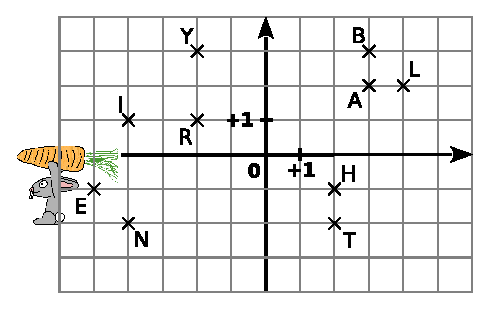
\includegraphics[width=7.2cm]{plan_carotte} \end{center}
Sur la grille ci-dessus, Monsieur Lapin aimerait dessiner l'itinéraire le conduisant à la carotte. Pour ce faire, il doit : 
\begin{itemize}
 \item Partir du point $L$ ; 
 \item Passer par tous les points de la figure une et une seule fois de telle sorte que deux points consécutifs aient une des deux coordonnées commune (abscisse ou ordonnée).
 \end{itemize}
 \begin{enumerate}
  \item Reproduis la figure et dessine le parcours ;
  \item En écrivant dans l'ordre de passage chacune des lettres rencontrées, quel mot trouves-tu ?
  \end{enumerate}
\end{exercice}


%%%%%%%%%%%%%%%%%%%%%%%%%%%%%%%%%%%%%%%%%%%%%%%%%%%%%%%%%%%%%%%%%%

\serie{Comparer}


\begin{exercice}[Nombres relatifs et droite graduée]
\begin{enumerate}
 \item Trace une droite graduée en centimètre.
 \item Sur cette droite graduée, place les points suivants :

\begin{center} $A (+ 3)$ ; $B (- 1)$ ; $C (- 3)$ ; $D (+ 5)$ ; $E (- 6)$. \end{center}
 \item En observant la droite graduée, range par ordre croissant les nombres suivants :
 
\begin{center} $+ 3$ ; $- 1$ ; $- 3$ ; $+ 5$ et $- 6$.\end{center}
 \end{enumerate}
\end{exercice}


\begin{exercice}
Compare les nombres suivants :
\begin{colenumerate}{2}
 \item $- 1$ et $+ 3$ ;
 \item $+ 4$ et $+ 6$ ;
 \item $- 6	$ et $- 2$ ;
 \item $- 2$ et $- 4$ ;
 \item $- 0$ et $+ 8$ ;
 \item $+ 3$ et $- 4$ ;
 \item $+ 4$ et $- 14$ ;
 \item $- 12$ et $- 18$ ;
 \item $- 4$ et 0 ;
 \item $- 212$ et $+ 212$.
 \end{colenumerate}
 \end{exercice}
 
 
\begin{exercice}
Compare les nombres suivants :
\begin{enumerate}
 \item $- 2,4$ et $- 2,3$ \dotfill ;	
 \item $+ 3,6$ et $- 6,3$ \dotfill ;
 \item $- 11,3$ et $- 9,7$ \dotfill	; 	
 \item 0 et $+ 3,9$ \dotfill ; 	
 \item $- 5,6$ et $- 5,60$ \dotfill ;	 	
 \item $+ 9,6$ et $+ 6,9$ \dotfill	;	
 \item $+ 32,57$ et $+ 32,507$ \dotfill ;	 	
 \item $- 125,64$ et $- 125,064$ \dotfill ;	 	
 \item $- 23,7$ et $+ 23,69$ \dotfill ;	
 \item $- 15,878$ et $- 15,8708$ \dotfill.
  \end{enumerate}
\end{exercice}
 
 
\begin{exercice}[Rangements]
Range par ordre croissant les nombres suivants :
\begin{enumerate}
 \item $+ 12$ ; $- 2$ ; $+ 1$ ; $+ 13$ ; $- 31$ ; $- 11$ ; $- 5$ ;
 \item $+ 15$ ; $- 9$ ; $- 8$ ; $+ 7$ ; $- 3$ ; $- 1$ ; $+ 6$ ; $+ 12$ ; $- 4$ ; $- 14$ ; 0 ;
 \item $- 25$ ; $+ 25,2$ ; $- 5,2$ ; $+ 2,5$ ; $- 3,2$ ; $+ 5,02$ ;
 \item $- 100,3$ ; $- 99,3$ ; $- 100,03$ ; $- 99,13$ ; $- 9,3$.
 \end{enumerate}
\end{exercice}
        
    
\begin{exercice}[Rangements (bis)]
Range par ordre décroissant les nombres suivants :
\begin{enumerate}
 \item $+ 3$ ; $- 15$ ; $+ 20$ ; $+ 15$ ; $- 100$ ; $- 25$ ; $+ 27$ :

 \dotfill
 
 \dotfill	
	
 \item $+ 12$ ; $- 15$ ; $+ 17$ ; $+ 21$ ; $- 13$ ; $- 17$ ; $- 5$ ; $- 2$ ; $+ 3$ :
 
 \dotfill

 \dotfill	
	
 \item $+ 3,5$ ; $- 20,39$ ; $- 12,03$ ; $+ 5,6$ ; $- 123,45$ :

 \dotfill
 
 \dotfill	
	
 \item $- 7,001$ ; $- 7,1$ ; $- 7,71$ ; $- 7,01$ ; $- 7,2$ ; $- 7,7$ :
 
 \dotfill
  
 \dotfill
 \end{enumerate}	
\end{exercice}


\begin{exercice}
Pour chaque nombre, complète par l'entier relatif qui suit ou qui précède :
\begin{colenumerate}{2}
 \item \ldots \ldots $< - 4$ ;
 \item $- 3 <$ \ldots \ldots ;
 \item $- 12 >$ \ldots \ldots ;
 \item \ldots \ldots $> - 15$ ;
 \item \ldots \ldots $< - 35$ ;
 \item \ldots \ldots $< + 125$. 
 \end{colenumerate}	
\end{exercice}


\begin{exercice}
Pour chaque nombre, recopie puis complète par l'entier relatif qui suit ou qui précède :
\begin{colenumerate}{2}
 \item \ldots \ldots $< - 2,3$ ;
 \item $- 1,1 <$ \ldots \ldots ;
 \item \ldots \ldots $> + 3,2$ ;
 \item $+ 5,71 >$ \ldots \ldots ;
 \item \ldots \ldots $> - 17,71$ ;
 \item $- 114,5 >$ \ldots \ldots ;
 \end{colenumerate}	
\end{exercice}


\begin{exercice}
Complète en intercalant un nombre entre les deux nombres proposés :
\begin{enumerate}
 \item $- 2 > \ldots \ldots > - 4$ ;
 \item $+ 5 < \ldots \ldots < + 6$ ;
 \item $- 14 > \ldots \ldots > - 17$ ;
 \item $0 > \ldots \ldots > - 2$ ;
 \item $+ 14 < \ldots \ldots < + 16$ ;
 \item $- 1,44 < \ldots \ldots < + 0,71$ ;
 \item $- 17,304 > \ldots \ldots > - 17,34$ ;
 \item $- 132,247 < \ldots \ldots < - 132,24$.
 \end{enumerate}
\end{exercice}


\begin{exercice}
Donne l'abscisse des points $A$, $B$ et $C$ :
\begin{center} 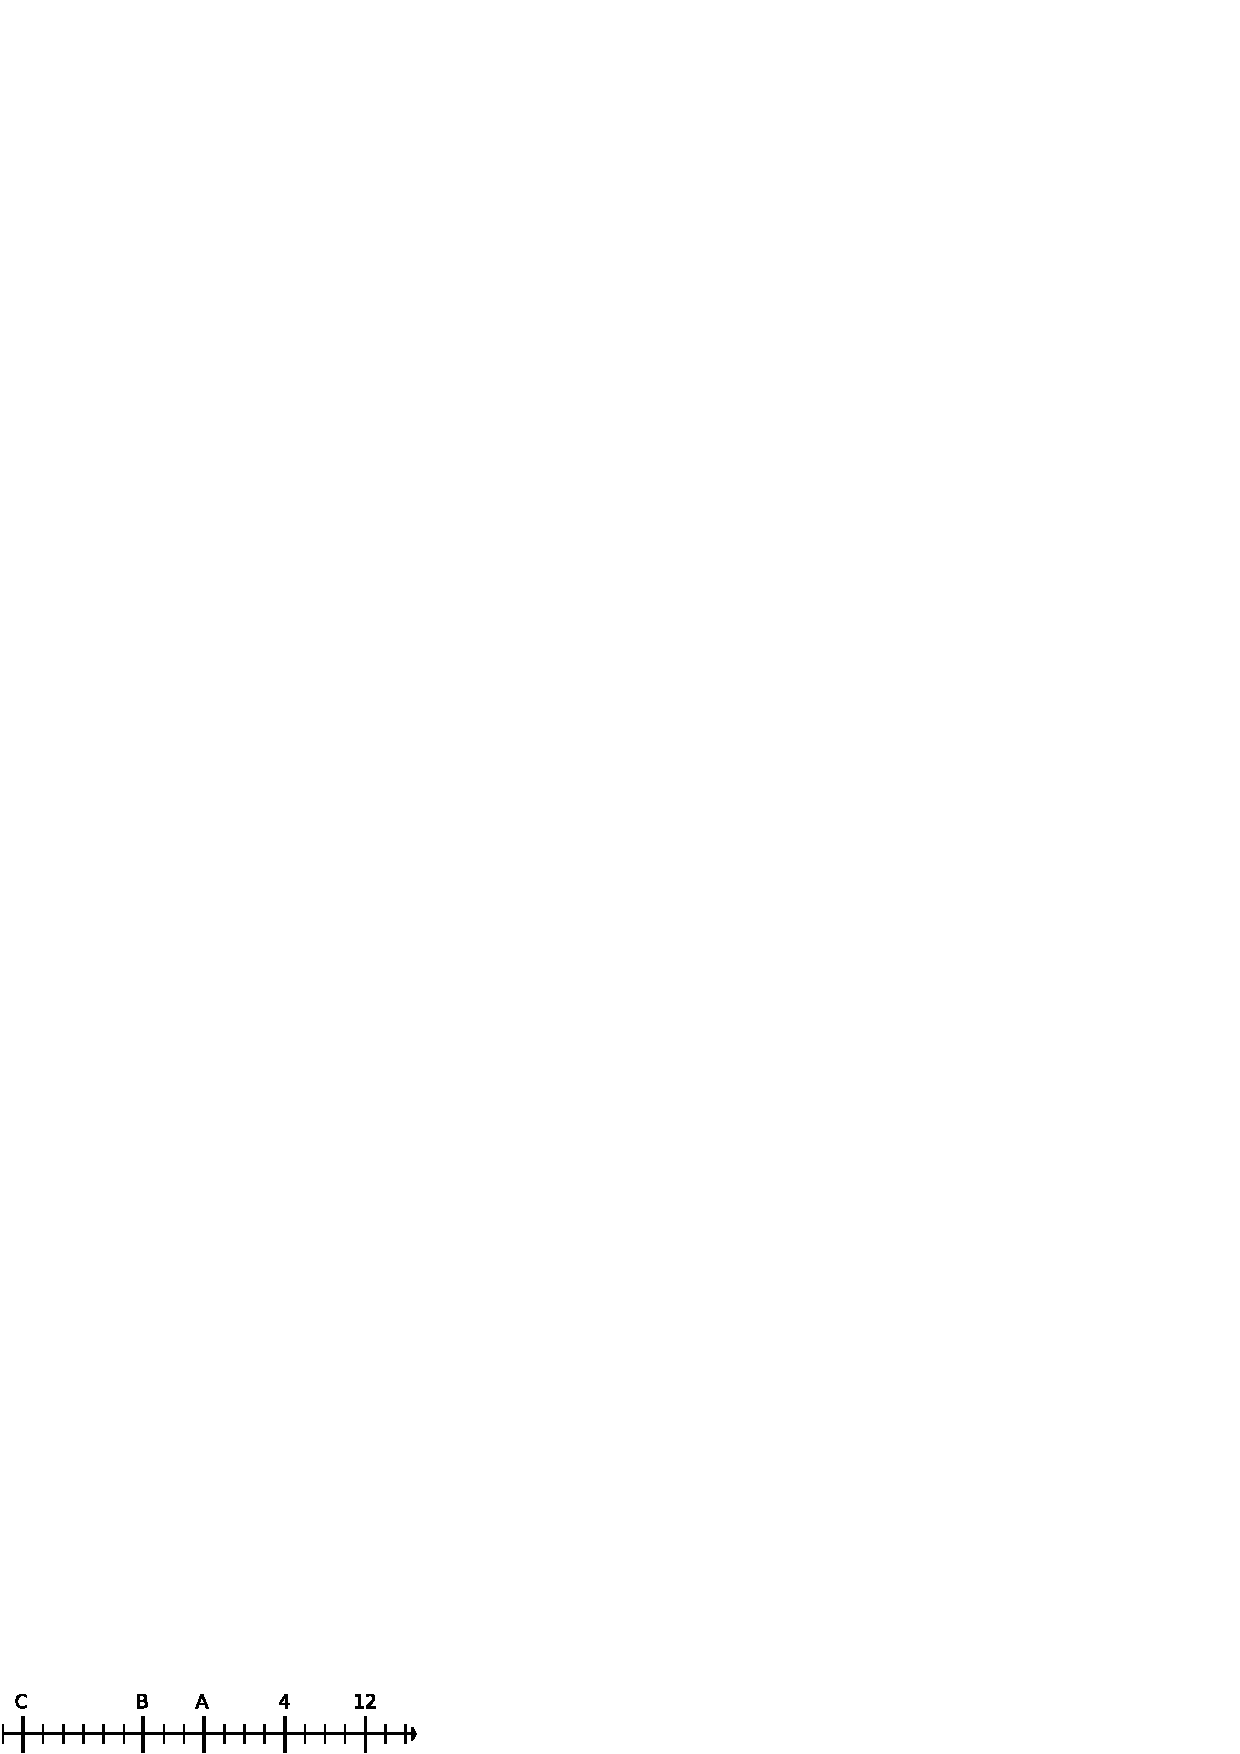
\includegraphics[width=6.7cm]{axeBAC} \end{center}

\dotfill

\dotfill
\end{exercice}


\begin{exercice}
Sur la droite ci-dessous, place les points $D(0,15)$, $E(- 0,1)$ et $F(0,55)$ :
\begin{center} 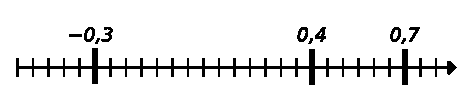
\includegraphics[width=7.1cm]{axe04} \end{center}
\end{exercice}


\begin{exercice}
Dans le repère ci-dessous, place les points suivants : 

$A(- 2 ; 1)$ ; $B(- 4 ; - 3)$ ; $C(5 ; - 1)$ ; $D(- 5 ; 0)$ ; $E(0 ; - 2)$.
\begin{center} 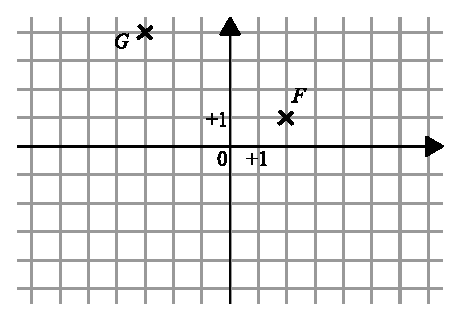
\includegraphics[width=6.9cm]{planGF} \end{center}
Donne ensuite les coordonnées des points $F$ et $G$.
\end{exercice}


\begin{exercice}
Complète par $<$ ou $>$ ou $=$ :
\begin{colitemize}{2}
 \item $+ 5,34 \ldots \ldots + 3,54$ ;
 \item $- 9,27 \ldots \ldots - 9,272$ ;
 \item $0,05 \ldots \ldots 1$ ;
 \item $+ 8,64 \ldots \ldots - 8,64$ ;
 \item $- 8,51 \ldots \ldots - 8,5$ ;
 \item $- 19,2 \ldots \ldots + 9,2$ ;
 \item $11,9 \ldots \ldots +11,9$ ;
 \item $- 14,39 \ldots \ldots - 14,4$ ;
 \item $- 3,14 \ldots \ldots - 1,732$ ;
 \item $- 0,99 \ldots \ldots - 0.909$.
 \end{colitemize}
\end{exercice}


\begin{exercice}
Range par ordre croissant les nombres suivants : \\[0.5em]
$+ 5,0$ ; $+ 2,7$ ; $- 2,6$ ; $- 3,1$ ; $+ 5,1$ ; $- 1,7$ ; $- 2,06$ ; $- 0,2$ :

 \dotfill

 \dotfill
\end{exercice}


\begin{exercice}
Range par ordre décroissant les nombres suivants : \\[0.5em]
$- 10,6$ ; $+ 14,52$ ; $- 8,31$ ; $+ 4,2$ ; $+ 14,05$ ; $- 14,5$ ; $- 8,003$ :

 \dotfill

 \dotfill
\end{exercice}


\begin{exercice}
Encadre chaque expression par deux nombres entiers consécutifs :
\begin{colitemize}{2}
 \item $\ldots < - 2,3 < \ldots$ ;
 \item $\ldots < + 4,2 < \ldots$ ;
 \item $\ldots < - 15,11 < \ldots$ ;
 \item $\ldots < - 0,14 < \ldots$ ;
 \item $\ldots < + 0,14 < \ldots$ ;
 \item $\ldots < - 0,98 < \ldots$ ;
 \item $\ldots < - 12,7 < \ldots$ ;
 \item $\ldots < - 0,003 < \ldots$ .
 \end{colitemize}
\end{exercice}


\begin{exercice}[Bulletin météo]
Voici quelques températures relevées à différents moments de la journée dans plusieurs villes de Suisse : \\[0.5em]
\begin{tabularx}{\linewidth}{|X|X|X|X|}
 \hline
 & Matin ($^\circ$C) & Midi ($^\circ$C) & Soir ($^\circ$C) \\\hline
 Lausanne & $- 4$ & $+ 1$ & $- 1$ \\\hline
 Delémont & $+ 2$ & $+ 4$ & $+ 3$ \\\hline
 Sion & $+ 5$ & $+ 9$ & $+ 6$ \\\hline
 Neuchâtel & $- 10$ & $- 6$ & $- 7$ \\\hline
 Fribourg & $- 2$ & $0$ & $- 3$ \\\hline
 Berne & $0$ & $+ 2$ & $- 2$ \\\hline
 Genève & $+ 4$ & $+ 7$ & $+ 2$ \\\hline
 \end{tabularx}
 \vspace{0.3cm}
\begin{enumerate}
 \item Range ces villes dans l'ordre croissant de  leur température du matin ;
 \item Range ces villes dans l'ordre décroissant de  leur température du soir ;
 \item Calcule la température moyenne de la journée pour Delémont, Sion et Genève.
 \end{enumerate}
\end{exercice}

